\documentclass[12pt,a4paper]{article}

\usepackage[left=1in,right=1in,top=1in,bottom=1in]{geometry}                % See geometry.pdf to learn the layout options. There are lots.
\usepackage[parfill]{parskip}    % Activate to begin paragraphs with an empty line rather than an indent
\usepackage{microtype} \hyphenpenalty=750
\usepackage{graphicx}
\usepackage{epstopdf} \DeclareGraphicsRule{.tif}{png}{.png}{`convert #1 `dirname #1`/`basename #1 .tif`.png}
% \usepackage[applemac]{inputenc}
\usepackage{booktabs}
% \usepackage{fancyhdr} \pagestyle{fancy} \chead{\hifibau} \cfoot{\thepage}
% \usepackage[english,ngerman]{babel}

\usepackage{siunitx}

\PassOptionsToPackage{hyphens}{url}\usepackage[colorlinks]{hyperref}
\usepackage{caption} \captionsetup{labelfont={sf,bf}, size=footnotesize}

\usepackage[superscript,biblabel]{cite}

% set format of document title
\usepackage{titling}
\pretitle{\begin{center}\Large\bfseries}
\posttitle{\end{center}\vspace{1em}}
\preauthor{\begin{center}\large}
\postauthor{\end{center}\vspace{1em}}
\predate{\begin{center}\large}
\postdate{\end{center}\vspace{1em}}

% set formats of section headings
\usepackage[explicit]{titlesec}
\titleformat{\title}{\centering}{\thesection.}{0.5em}{\MakeUppercase{#1}}
%\titleformat{\section}{\centering}{\thesection.}{0.5em}{\MakeUppercase{#1}}
\titleformat{\section}{}{\thesection.}{0.5em}{\MakeUppercase{#1}}
%\titleformat{\subsection}[runin]{\slshape}{\thesubsection.}{0.5em}{#1. }
\titleformat{\subsection}{\slshape}{\thesubsection.}{0.5em}{#1 }
\titleformat{\subsubsection}[runin]{\slshape}{\thesubsubsection.}{0.5em}{#1. }
 
\usepackage[T1]{fontenc} \usepackage[scaled=.90]{helvet} \renewcommand{\familydefault}{\sfdefault} \usepackage[helvet]{sfmath}

\newcommand{\Ohm}{\ensuremath{\Omega}}
\sisetup{detect-all} % tell siunitx to detect font stuff


% \setlength{\columnsep}{0.75cm} 

\graphicspath{{figures/}}

% \interfootnotelinepenalty=10000

\providecommand{\figr}[1]{Fig.~\ref{fig:#1}}
\providecommand{\figlabel}[1]{\label{fig:#1}}
\providecommand{\tabl}[1]{Tab.~\ref{tab:#1}}
\providecommand{\tablabel}[1]{\label{tab:#1}}
\providecommand{\secn}[1]{Sec.~\ref{sec:#1}}
\providecommand{\seclabel}[1]{\label{sec:#1}}


%% define formats of section and subsection etc. headings:
%    \makeatletter
%    \def\section{\@startsection{section}{1}%
%    \z@{.7\linespacing\@plus\linespacing}{.5\linespacing}%
%%    {\normalfont\bfseries\centering}}
%    {\Large\centering}}
%    
%    \def\subsection{\@startsection{subsection}{2}%
%    \z@{.5\linespacing\@plus.7\linespacing}{-.5em}%
%%    {\normalfont\bfseries\itshape}}
%    {\normalfont\itshape}}
%    
%    \def\subsubsection{\@startsection{subsubsection}{3}%
%    \z@{.5\linespacing\@plus.7\linespacing}{-.5em}%
%%    {\normalfont\bfseries}}
%    {\normalfont\itshape}}
%    
%    \makeatother






\title{The Open-Source Directly-Heated Triode \\ Electrostatic Headphone Amplifier \\ (OSDEHA)}
\author{Matthias Brennwald}
\date{THIS DOCUMENT IS UNDER CONSTRUCTION!\\ Draft Version \today}

\begin{document}

% \twocolumn[\maketitle]

\maketitle

\emph{Warning: This DIY project involves high voltage. Individuals utilizing the information provided must possess expert knowledge, adhere to stringent safety precautions, and accept all risks associated with electrical work. The authors and contributors of this project expressly disclaim any liability for injuries or damages arising from the use or misuse of this information.}


\section{Overview}

This document describes an audio amplifier for electrostatic headphones. The design of the amplifier is targeted at DIY builders and is published as open hardware (see \secn{license}).

Electrostatic headphones operate on audio signals characterized by high voltage and low current. This is the domain of vacuum tubes, making them most suitable as drivers for electrostatic headphones.  While there exist a number of tube amplifiers for electrostatic headphones, many of these designs do not utilize directly-heated triodes (DHTs), which exhibit outstanding linearity and sound quality.\par

The OSDEHA uses DHT tubes for its output stage and implements the following design goals:
\begin{itemize}
\item The audio output is taken directly from the anodes of the DHT output tubes. There are no transformer or capacitors to transfer the power to the headphones.
\item The amplifier input takes balanced input at signal levels of modern audio sources (mostly DACs these days).
\item The design prioritizes the quality of audio reproduction and electronic design rather than on low cost.
\item The amplifier should be reasonably compact, and all units and boards should fit in one single chassis.
\end{itemize}

There is a public discussion thread of the OSDEHA at diyAudio\cite{osdeha_p1}. 

\section{Amplifier Circuit}

\subsection{Driving electrostatic headphones} \seclabel{estat_drive}

Electrostatic headphones utilize three electrodes: two fixed outer electrodes (stators) and a movable central electrode (diaphragm). The diaphragm is biased at a high voltage relative to the stators. The audio signal is applied to the stators in opposite polarities, creating an electric field that controls the movement of the charged diaphragm. For accurate sound reproduction, the electrostatic forces acting on the diaphragm must be proportional to the applied audio signal. To avoid distortion of the audio output from the headphone, the charge on the diaphragm therefore needs to be maintained constant.

The electrical impedance of electrostatic headphones is primarily determined by the capacitance of the two stators, which is typically around \SI{100}{pF}\cite{osdeha_p3}.

The voltage swing to drive the stators depends on the headphone sensitivity and the desired sound pressure level. An experiment using various genres of well-recorded music indicated that an undistorted \SI{1.3}{kV} peak-to-peak swing of the bipolar output is desirable (i.e., \SI{650}{V} peak-to-peak at each stator)\cite{osdeha_p8}. The corresponding current swing measured in this experiment was approximately \SI{4}{mA}, but driving the \SI{100}{pF} load to full output at \SI{20}{kHz} and higher necessitates larger peak currents, around \SI{20}{mA}\cite{osdeha_p2}.

% With a balanced line-level input ($2\times\SI{3.5}{V}$ peak-to-peak), the required voltage gain of the amplifier is $1300/(2\times 3.5) = 185\times$, or \SI{+45}{dB}.

\subsection{Output Stage}\seclabel{outputstage}

\figr{OPS_concept} shows the conceptual layout of the OSDEHA. The output stage uses two DHTs in a push-pull arrangement to provide the symmetric, bipolar output needed to drive electrostatic headphones. For efficient transfer of the audio power to the headphones, the AC impedance of the anode loads must be larger than that of the headphones (several \unit{M\Ohm}). This cannot be implemented with passive anode-load resistors, so active constant-current sources (CCSs) are used in this position. The CCS loads also improve the linearity and voltage gain of the amplifier, and suppress ripple and noise from the B+ rails.

\begin{figure}
\begin{center}
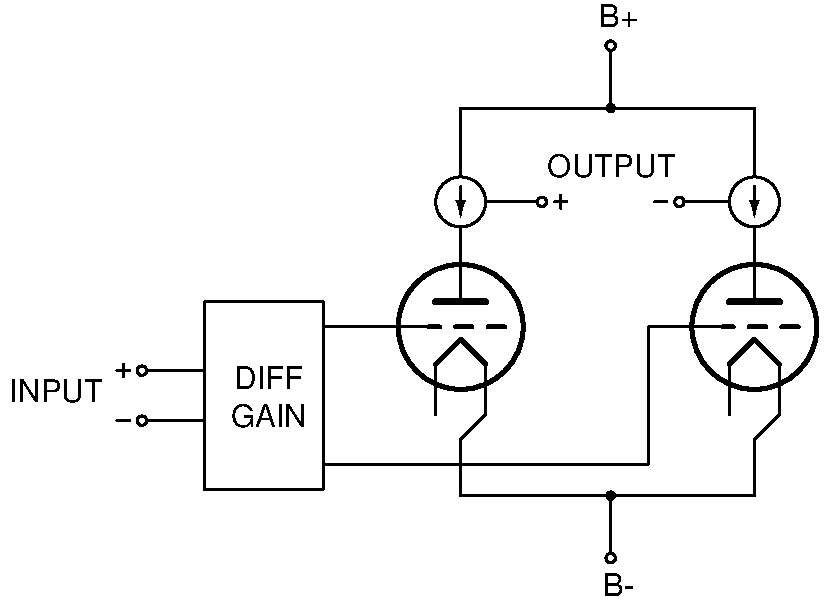
\includegraphics[width=0.7\textwidth]{OPS_concept.pdf}
\caption{Conceptual layout of the OSDEHA: differential input and gain stage, push-pull DHT output stage.}
\figlabel{OPS_concept}
\end{center}
\end{figure}

The choice of the output tube type is determined by the drive requirements for the headphone, as described in \secn{estat_drive}. Since the two tubes are in series with the headphone, each tube contributes half of the total voltage swing. Each tube needs to swing \SI{\pm325}{V} at a \SI{20}{mA} bias. Additionally, to emphasize the ``DHT sound,'' the DHT output stage should contribute as much voltage gain as possible to the overall gain of the amplifier.

Several DHT tube types were considered for the OSDEHA\cite{osdeha_p9,osdeha_whichDHT}. In particular:

\begin{itemize}
\item The 841/VT-51 tube has a gain of 30$\times$ and can be biased up to \SI{425}{V}. However, at the operating point required for the OSDEHA, the 841 tends to operate at a positive grid voltage, which leads to grid current draw. Moreover, these tubes are relatively scarce.
\item The 20B tube is a modern design with a gain of 20$\times$ and can be biased up to about \SI{500}{V}. However, these tubes are quite large (approximately the size of a beer bottle) and are manufactured only in small quantities by a single producer (Emissionlabs), making their long-term availability uncertain.
\item The family of the 801/801A/VT-62 and 10Y/VT-25 types\cite{aasyl_801types} provide a gain of 8$\times$. The 801 can be biased up to \SI{500}{V}, while the 10Y should not be biased above \SI{450}{V}. These tubes are available as new-old-stock and from new production.
\end{itemize}

From a technical standpoint, the high gain of the 20B would would make this tube an interesting option. However, due to concerns about the long-term availability of the 20B, the 801/10Y family of tubes is considered a more practical choice for the OSDEHA design.

\figr{801A_curves} shows the characteristic curves measured from the 801A tube (the 10Y/VT-25 are equivalent) with the load line of a \SI{20}{mA} CCS. The anode DC bias is set at \SI{420}{V}, corresponding to a grid bias of approximately \SI{-34}{V}. This bias point facilitates an anode voltage swing of \SI{\pm325}{V} within the linear operating range of the tube. The grid voltage does not exceed +\SI{10}{V}, where the grid current has been measured to stay well below \SI{1}{mA}. With the anode voltage close to GND, the B- voltage is \SI{-420}{V}, and B+ is \SI{+420}{V} for symmetry.

\begin{figure}
\begin{center}
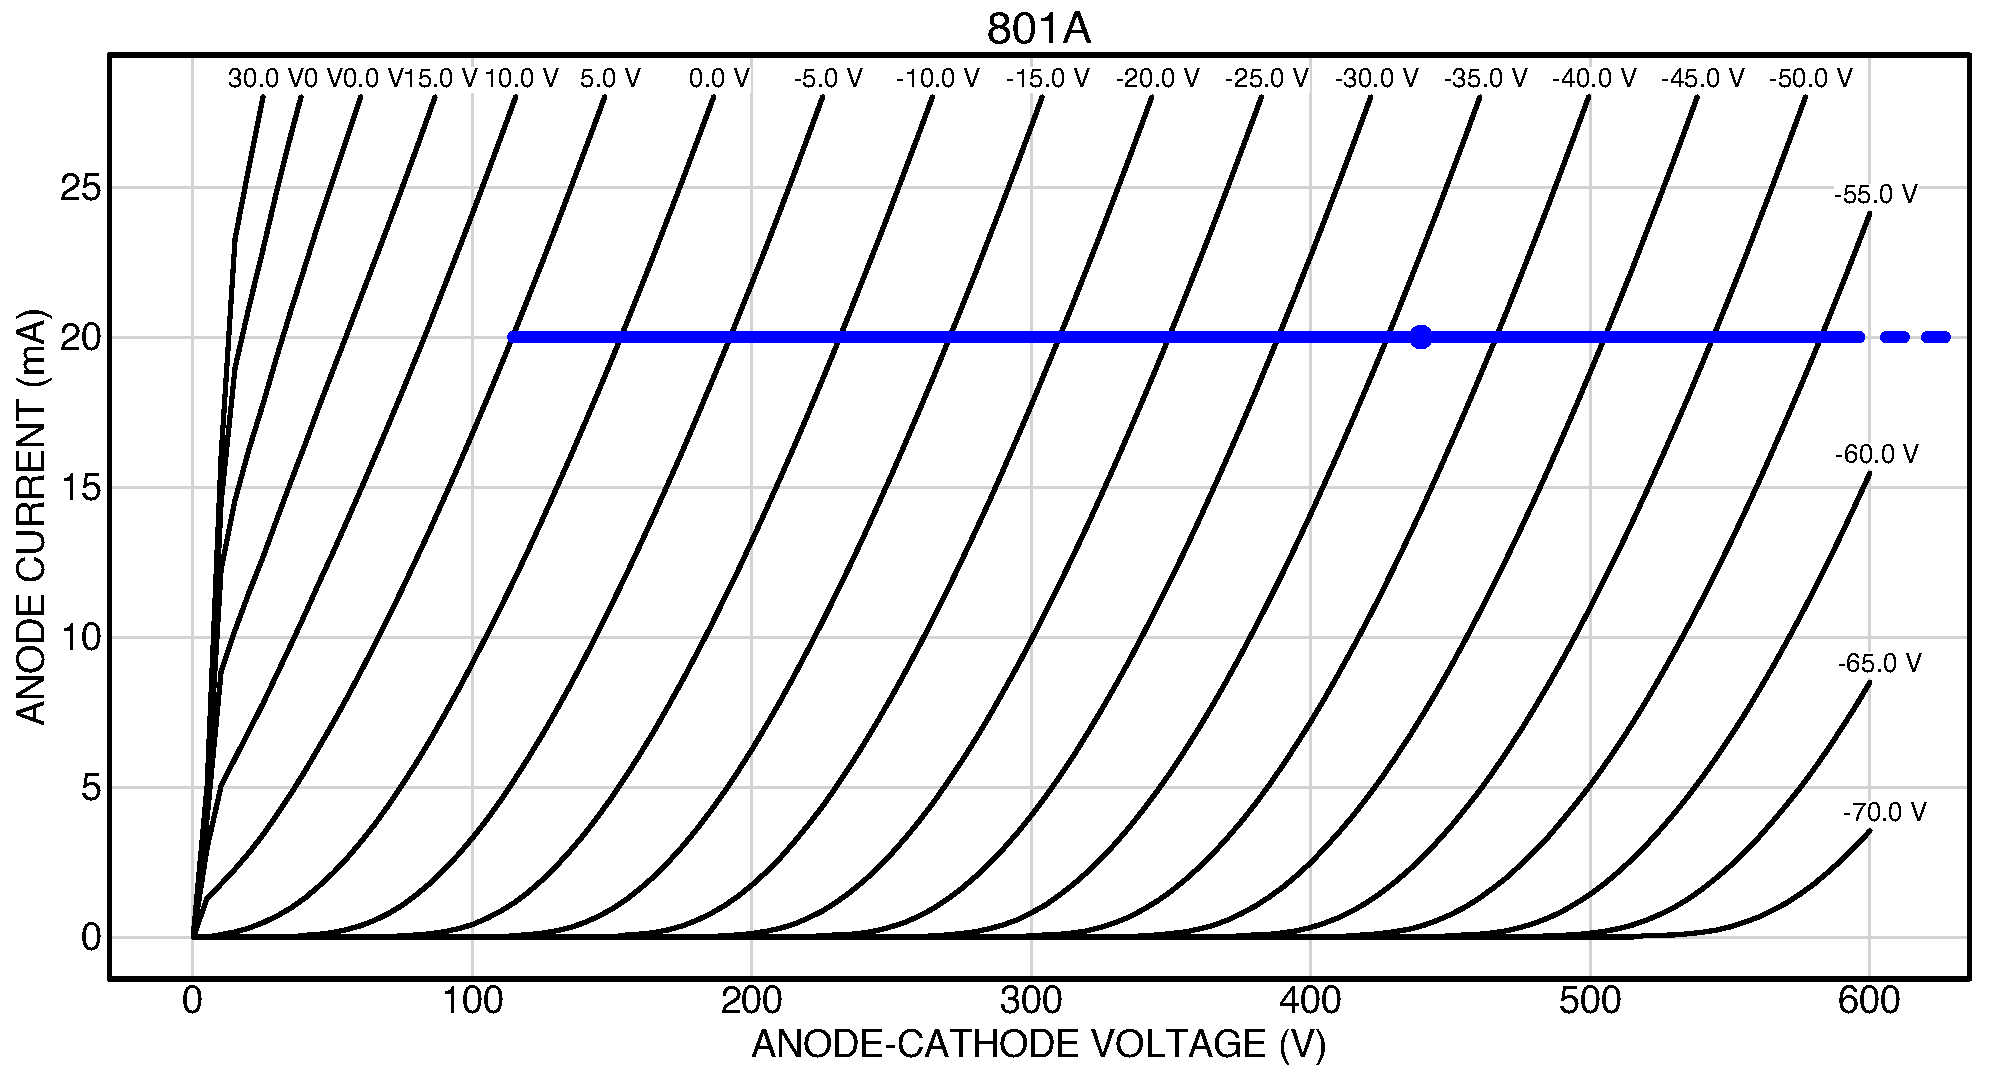
\includegraphics[width=0.8\textwidth]{801A_curves.pdf}
\caption{Characteristic curves measured from an 801A DHT, with a DC bias point at \SI{420}{V} and \SI{20}{mA}, and a constant-current loadline showing \SI{\pm325}{V} anode swing (blue).}
\figlabel{801A_curves}
\end{center}
\end{figure}

\figr{activeload_concept} shows the simplified circuit of the CCSs used to load the anodes of the DHT output tubes. This circuit works as a CCS in the audio/AC domain only, while it outputs a fixed voltage in the DC domain. In both cases, the FET Q1 controls the output of the circuit to the anode, while the depletion-mode FET Q2 drops most of the voltage from B+ and decouples Q1 from any noise or ripple that may be present in the B+ supply.\par

\begin{figure}
\begin{center}
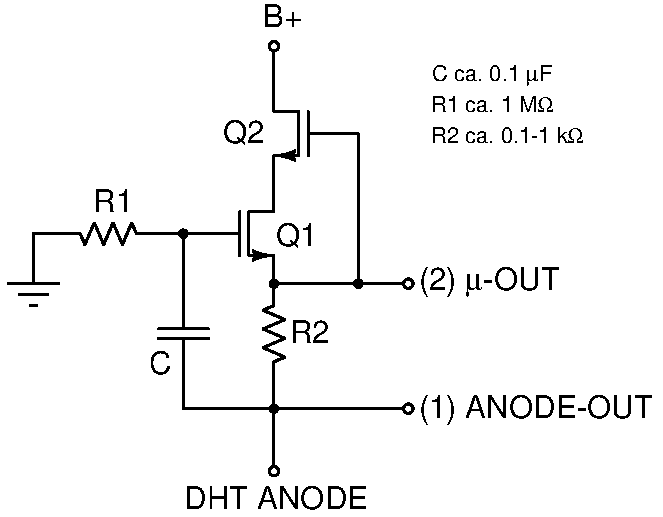
\includegraphics[width=0.5\textwidth]{activeload_concept.pdf}
\caption{Circuit of the active load (AC coupled CCS, simplified).}
\figlabel{activeload_concept}
\end{center}
\end{figure}

In the audio/AC domain, the gate of Q1 is tied to the anode through capacitor C. Q1 mirrors any AC variation of the anode voltage from the gate to its source pin. This maintains a constant voltage between the Q1 source and the DHT anode, and thereby keeps the current through R2 constant. If the headphone stator is driven directly by the DHT anode (output 1 in \figr{activeload_concept}), this current is shared between the DHT and the stator. Therefore, the current flowing through the DHT will exhibit a slight variation in response to the AC current consumed by the stator. This variation is typically less than \SI{4}{mA}\cite{osdeha_p8}, which is considerably less than the DC bias current. The general concept for the operating point illustrated in \figr{801A_curves} therefore remains valid. However, instead of taking the audio output from the DHT anode, the stator can also be connected to the $\mu$-output (output 2 in \figr{activeload_concept}). In this $\mu$-follower configuration\cite{pimm_ccs,kimmel_mustage}, the stator draws its current directly form Q1, not through R2.\cite{muresistorvalue} This restores the constant-current operation of the DHT tube with a flat load line as shown in \figr{801A_curves}.\par

In the DC domain, the gate pin of the FET Q1 is grounded via R1, and the source pin is therefore fixed at $-V_{\rm GS,0}$. This biases the anode at a small negative DC voltage determined by $V_{\rm GS,0}$ and the DC drop across R2. This maintains a stable DC voltage at the amplifier outputs despite any thermal drift or aging of the DHT tubes.


\subsection{Input Stage}\seclabel{inputstage}

The task of the input stage is to amplify the balanced input signal ($2 \times \SI{3.5}{V}$ peak-to-peak) to drive the DHT grids ($2 \times \SI{86}{V}$ peak-to-peak). To this end, a voltage gain of $86 / 3.5 = 25\times$ is needed.\par

Following the lines of the output stage, the differential input stage is designed as long-tailed pair (LTP)\cite{valvewizard_LTP} using tubes with triode characteristics. The ``tail'' is implemented as a CCS to maximize linearity and voltage gain of the LTP (\figr{IPS_concept}).

\begin{figure}
\begin{center}
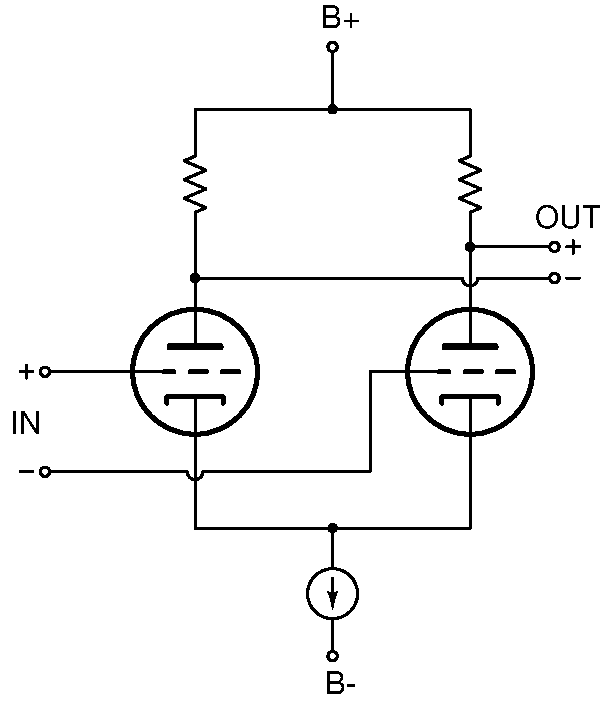
\includegraphics[width=0.6\textwidth]{IPS_concept.pdf}
\caption{Input stage (simplified).}
\figlabel{IPS_concept}
\end{center}
\end{figure}

The E180F or 6E5P tubes connected as triodes provide suitable gain and offer very linear amplification\cite{bartola_thdbenchmark,millett_pentodes,klausmobile_testerfiles}. However, the E180F tends to be microphonic\cite{osdeha_p23}, and its linearity was found to be slightly inferior to that of the 6E5P\cite{osdeha_p32}, making the 6E5P the preferred choice for the LTP input stage. Each triode unit is biased at \SI{10}{mA} and \SI{170}{V} anode-cathode voltage with a \SI{25}{k\Ohm} load resistor, which provides for more than \SI{\pm100}{V} anode AC swing. (\figr{6E5P_curves}).

The LTP input stage is capacitor coupled to the grids of the output DHTs. A suitable capacitor will not have any measureable effect on the audio signal\cite{bateman_caps_distortion} as long as there is no substantial current flow across the capacitor\cite{aiken_farting_out}. The DHT grids are therefore driven by FETs configured as source followers. The DC bias voltage for the DHT output tubes is applied to the gates of the FETs to guarantee stable bias even if the DHT grids are driven into grid current.

\begin{figure}
\begin{center}
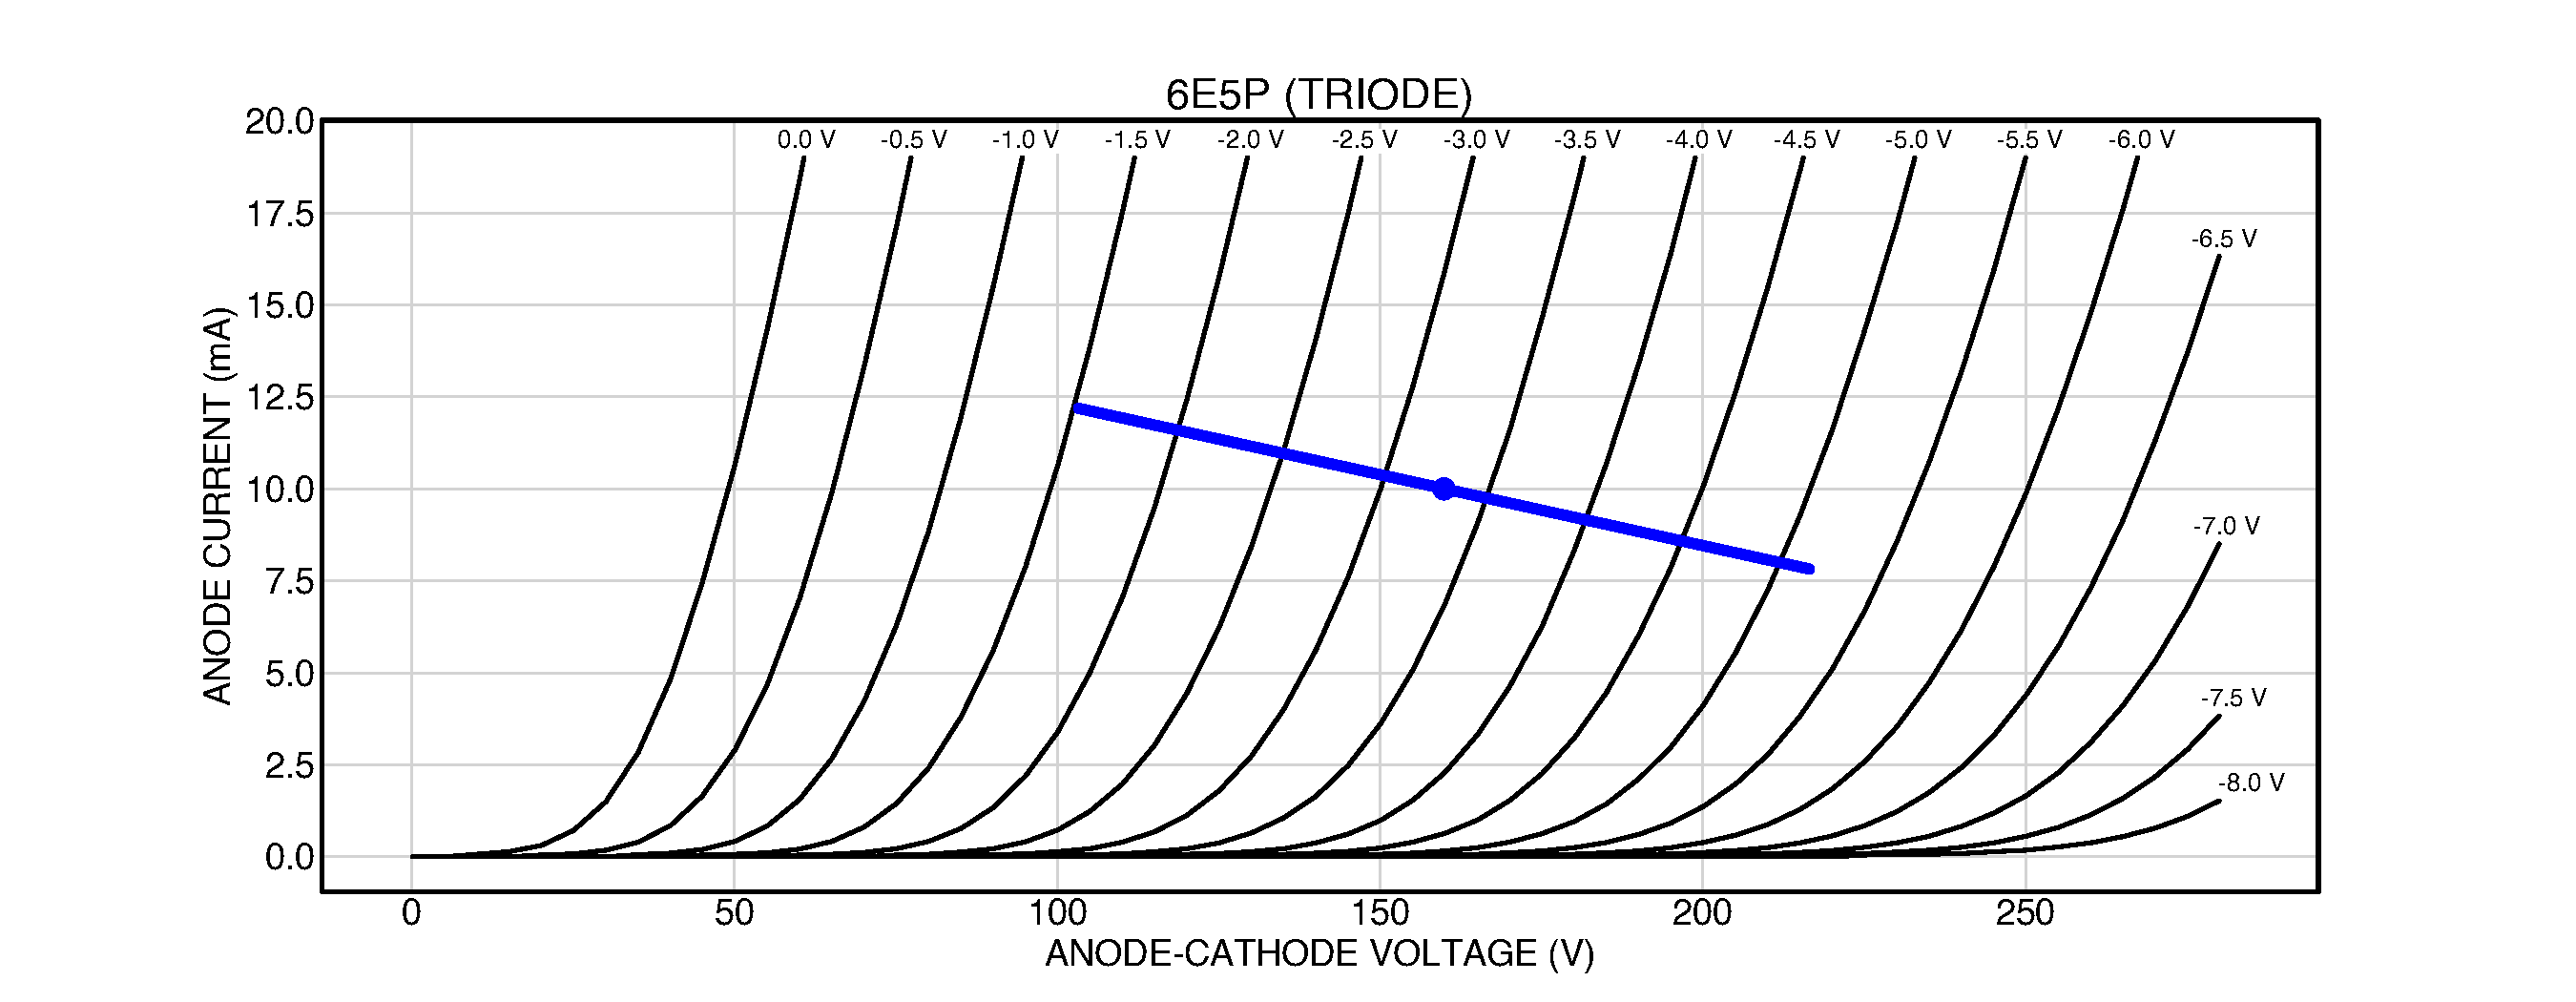
\includegraphics[width=0.8\textwidth]{6E5P_curves.pdf}
\caption{Characteristic curves measured from a triode-connected 6E5P tube, with a \SI{25}{k\Ohm} load line and DC bias at \SI{170}{V} and \SI{10}{mA}.}
\figlabel{6E5P_curves}
\end{center}
\end{figure}


\section{Power supplies}

\subsection{High voltage supplies (B+, B-, B2-)}

\subsection{Bias}

\subsection{DHT filament supply}

\subsection{Heater supply for input stage}


\section{Putting the pieces together}

FULL SCHEMATICS AND DESCRIPTION




\section{Mechanical construction}

HEATSINKS, CHASSIS, ETC.


\section{Bring-up and initial adjustments}

Building, testing, and adjusting the OSDEHA is best done step by step as described below. Use a variac to slowly bring up the circuits. It's recommended to built, install and fully test one amplifier board before working on the second one. Before working on the circuits, reset the variac to zero, switch off power, and wait for all capacitors to discharge such that no (high) voltages are left anywhere in the circuits.

\subsection{Power supply}
\begin{itemize}
\item Assmemble the power-supply boards. Install the boards and transformers in the amplifier chassis. Connect the primary windings of the transformers to the mains inlet and power switch of the amplifier chassis.
\item Connect the amplifier to mains power through a variac (set the variac to zero before plugging it to the wall outlet).
\item Connect transformer secondaries of heater supply. Then slowly ramp up the variac and confirm the heater supply works as expected. Also confirm the function of the HV delay relay.
\item Connect transformer secondaries of the DHT filament supply. Install dummy resistor at the filament connections and then slowly ramp up the variac to confirm if the heater supply works as expected, then remove the dummy resistors.
\item Connect the transformer secondaries of the high-voltage supplies and install dummy resistors at their outputs. Slowly ramp up the variac. Confirm and adjust HV output voltages. Also check the diaphragm bias voltage output (note: the internal resistance of the volt meter will load down the bias output, resulting in a low voltage reading).
\item Remove the dummy resistors from the high-voltage supplies.
\end{itemize}


\subsection{Amplifier input stage}
\begin{itemize}
\item Assmemble the amplifier board, install the board in the amplifier chassis, and set up the wire connections to volume pot and the connectors on the chassis. Install the tubes of the input stage, but do \emph{not} yet install or connect the DHT tubes of the output stage.
\item Connect the heater supply to the amplifier board. Slowly ramp up the variac and confirm the functioning of the heaters of the input-stage tubes.
\item Connect the high-voltage supplies to the amplifier board. Slowly ramp up the variac and confirm the correct DC bias of input stage tubes (anode voltages, CCS tail currents) and the DC bias currents of the buffer stages. Depending on the characteristics of your specific DN2540 parts it may be necessary to adjust the bias points by using different values for the CCS sense resistors.
\item Apply an AC test signal to the amplifier input and switch on power. Follow the signal along the circuit and confirm correct output from the buffer stage.
\end{itemize}


\subsection{Amplifier output stage}
\begin{itemize}
\item With the output tubes still disconnected from the amplifier, adjust DC grid bias of output tubes to the most negative value.
\item Disconnect the high-voltage supplies from the amplifier board, connect the DHT filament supply, and connect the DHT output tubes to the amplifier. Slowly ramp up the variac and adjust the filament voltage to the target value.
\item Reconnect the high-voltage supplies to the amplifier board and slowly ramp up the variac. Monitor the DC bias current of each output tube by reading the voltage across the mu-resistors. Adjust the DC grid bias until the targeted DC bias points are achieved. Let the amplifier warm up and readjust DC bias as necessary. Also monitor the filament voltages during warmup, and readjust if necessary.
\item Apply an AC test signal to the amplifier input and check for correct output from the amplifier.
\end{itemize}



\section{Specifications and test results}

TESTS AND MEASUREMENTS

OUTPUT BEFORE CLIPPING

FREUQNECY RESPONSE

DISTORTION MEASUREMENTS (THD, IMD, SPECTRA)


\section{License information} \seclabel{license}
Copyright Matthias Brennwald 2024.                                                    

The OSDEHA is Open Hardware and is licensed under the CERN-OHL-S v2 or any later version.

You may redistribute and modify this source and make products using it under the terms of the CERN-OHL-S v2 (\url{https://ohwr.org/cern_ohl_s_v2.txt}).

This source is distributed WITHOUT ANY EXPRESS OR IMPLIED WARRANTY, INCLUDING OF MERCHANTABILITY, SATISFACTORY QUALITY AND FITNESS FOR A PARTICULAR PURPOSE. Please see the CERN-OHL-S v2 for applicable conditions.

Source location: \url{https://github.com/mbrennwa/OSDEHA}

As per CERN-OHL-S v2 section 4, should You produce hardware based on this source, You must where practicable maintain the Source Location visible on the external case of the OSDEHA or other products you make using this source.            


% list of references
\bibliographystyle{unsrt}
\bibliography{OSDEHA_documentation}


\end{document}
